% `advanced_example.tex', an advanced example employing the AIAA class
% plus other third-party LaTeX packages.
%
% For a bare-bones usage, see `template.tex'.
%
% Typical processing for PostScript (PS) output:
%
%  latex advanced_example
%  bibtex advanced_example  (bibliography)
%  makeindex -s nomencl.ist -o advanced_example.gls advanced_example.glo
%                            (nomenclature)
%  latex advanced_example   (repeat as needed to resolve references)
%
%  xdvi advanced_example    (onscreen draft display)
%  dvips advanced_example   (postscript)
%  gv advanced_example.ps   (onscreen display)
%  lpr advanced_example.ps  (hardcopy)
%
% With the above, only Encapsulated PostScript (EPS) images can be used.
%
%
%  pdflatex advanced_example
%  bibtex advanced_example    (bibliography)
%  makeindex -s nomencl.ist -o advanced_example.gls advanced_example.glo
%                              (nomenclature)
%  pdflatex advanced_example  (repeat as needed to resolve references)
%
%  acroread advanced_example.pdf  (onscreen display)
%
% If you have EPS figures, you will need to use the epstopdf script
% to convert them to PDF because PDF is a limmited subset of EPS.
% pdflatex accepts a variety of other image formats such as JPG, TIFF,
% PNG, and so forth -- check the documentation for your version.
%
% If you do *not* specify suffixes when using the graphicx package's
% \includegraphics command, latex and pdflatex will automatically select
% the appropriate figure format from those available.  This allows you
% to produce PS and PDF output from the same LaTeX source file.
%
% To generate a large format (e.g., 11"x17") PostScript copy for editing
% purposes, use
%
%  dvips -x 1467 -O -0.65in,0.85in -t tabloid advanced_example
%
% For further details and support, read the Users Manual, aiaa.pdf.

\documentclass[]{aiaa-tc}% insert '[draft]' option to show overfull boxes

 \usepackage{varioref}%  smart page, figure, table, and equation referencing
 \usepackage{wrapfig}%   wrap figures/tables in text (i.e., Di Vinci style)
 \usepackage{threeparttable}% tables with footnotes
 \usepackage{dcolumn}%   decimal-aligned tabular math columns
  \newcolumntype{d}{D{.}{.}{-1}}
 \usepackage{nomencl}%   nomenclature generation via makeindex
  \makeglossary
 \usepackage{amssymb,amsmath}
 \usepackage{subfigure}% subcaptions for subfigures
 \usepackage{subfigmat}% matrices of similar subfigures, aka small mulitples
 \usepackage{fancyvrb}%  extended verbatim environments
 \fvset{fontsize=\footnotesize,xleftmargin=2em}
 \usepackage{lettrine}%  dropped capital letter at beginning of paragraph
%  \usepackage[dvips]{dropping}% alternative dropped capital package
 \usepackage[colorlinks]{hyperref}%  hyperlinks [must be loaded after dropping]
 \usepackage{float}
 \usepackage{longtable,booktabs,tabularx}
 % \restylefloat{table}
 \usepackage{graphicx}
 \usepackage{caption}
 \usepackage{siunitx}
 \usepackage{multicol}
 \usepackage{indentfirst}
 \usepackage{environ}
 \usepackage[labelfont=bf]{caption}
 \usepackage{multirow}
 \usepackage{setspace}
%  \graphicspath{{./figs/}}
 \usepackage[sort, numbers]{natbib}

\usepackage{bm}
%\title{Conceptual Design of an Extremely Short Takeoff and Landing Aircraft (using GPkit/for Urban Air Mobility)}
\title{Conceptual Design of an Urban Air Mobility System using GPkit}
 \author{
  Chris Courtin\thanks{Graduate Student, Aeronautics and Astronautics Engineering, MIT, 77 Mass Ave, Cambridge MA, 02139, AIAA Member.}, 
  Michael Burton\thanks{Graduate Student, Aeronautics and Astronautics Engineering, MIT, 77 Mass Ave, Cambridge MA, 02139, AIAA Student.}, 
  Patrick Butler\thanks{Graduate Student, Aeronautics and Astronautics Engineering, MIT, 77 Mass Ave, Cambridge MA, 02139, AIAA Student.}, 
  Alison Yu\thanks{Graduate Student, Aeronautics and Astronautics Engineering, MIT, 77 Mass Ave, Cambridge MA, 02139, AIAA Student.}, 
  John Hansman\thanks{T. Wilson Professor, Aeronautics and Astronautics Engineering, MIT, 77 Mass Ave, Cambridge MA, 02139, AIAA Student.} \\
  {\normalsize\itshape
   Massachusetts Institute of Technology, Cambridge, 02139, USA}\\
 }

 % Data used by 'handcarry' option
 \AIAApapernumber{YEAR-NUMBER}
 \AIAAconference{Conference Name, Date, and Location}
 \AIAAcopyright{\AIAAcopyrightD{YEAR}}

 % Define commands to assure consistent treatment throughout document
 \newcommand{\eqnref}[1]{(\ref{#1})}
 \newcommand{\class}[1]{\texttt{#1}}
 \newcommand{\package}[1]{\texttt{#1}}
 \newcommand{\file}[1]{\texttt{#1}}
 \newcommand{\BibTeX}{\textsc{Bib}\TeX}
 \usepackage{hyperref}
 \hypersetup{citecolor = blue}

\begin{document}

\graphicspath{{./figs/}} 
\maketitle

\begin{abstract}
    The conceptual design of an Urban Air Mobility (UAM) system that features electric Extremely Short Takeoff and Landing (ESTOL) vehicles is presented.  An overview is given of the system constraints that must be incorporated into the design of the vehicle.  The system-wide advantages and limitations of ESTOL aircraft are discussed, for both near- and far-term system implementations.  A detailed vehicle sizing model is developed using GPkit, a robust optimization framework.  This model is used to determine feasible boundaries on required runway size, vehicle range, and the sensitivity of the vehicle design to high-level mission parameters such as speed and number of passengers.  Key unique drivers of the vehicle design are identified.  The impact of distributed electric propulsion (DEP) is assessed.  The performance of the vehicle compared to a comparable Vertical Takeoff and Landing (VTOL) vehicle is analyzed, with currently available technology and forecasted future technology.   The infrastructure requirements (runway size, approach paths, etc.) needed to support ESTOL operations are assessed according to current regulations.  Two major urban areas (Boston and Los Angeles) are presented as case studies to show where this infrastructure could be feasibly located.  Key challenges and risks to implementation are discussed.  


\end{abstract}

\section*{Nomenclature}

\begin{multicols}{2}
\small

\begin{tabbing}
  XXXXXXX \= \kill% this line sets tab stop
$A$ \> wing aspect ratio \\
$b$ \> wing span \\ % [ft] \\
$c$ \> wing chord \\ %[m] \\
 \end{tabbing}

\end{multicols}
% \printglossary% creates nomenclature section produced by MakeIndex

\section{Introduction}
We would like to take this opportunity to distance ourselves from that Brian Seeley guy, and consider this whole urban air mobility concept with some objectivity. 

\paragraph{Current Technology} Extremely Short Takeoff and Landing (ESTOL) aircraft are not a new concept.  The Helio Courier, first built in the late 1940s, had demonstrated takeoff and landing distances from 100-300ft.  Highly experienced bush pilots are able to achieve landing distances on the order of single aircraft lengths.  Building aircraft that can operate of extremely short runways is clearly technologically feasible (whether it is commercially viable is an altogether different question).  Nevertheless, ESTOL aircraft technology has not found wide adoption outside of the relatively small community of pilots who routinely fly to remote, relatively unimproved landing areas.   There are inherent challenges in taking existing ESTOL aircraft and using them for operations near major urban areas, which are a result of the design penalties that ESTOL capability drove on the vehicles.  
For example, current ESTOL vehicles achieve their short field performance through a combination of low wing loading, high power-to-weight, and extensive use of high-lift systems.  The low wing loading means that both maximum and best cruise speeds are fairly low.  Additionally, it makes the vehicles highly sensitive to gusts and turbulence, an important consideration for passenger operations.   The high-lift systems required are also complex (except for impractically low wing loadings), which adds a weight and cost penalty to these vehicles.  Depending on the powerplant type used, the need for high power at takeoff may also reduce the efficiency at the nominal cruising point.  More significantly, these high-power engines generated substantial noise on takeoff; a primary consideration when operating near urban areas. 

\paragraph{Key Enabling Technologies} The introduction of new electric aircraft technologies has the potential to change the paradigm of current ESTOL aircraft and make them practical for use in an Urban Air Mobility (UAM) setting.   In the case of an all-electric aircraft, the reduction in noise through the use of batteries and an electric motor is one key area of improvement.  Another is the use of blown lift with distributed electric propulsion, in a configuration similar to the NASA X-57 Maxwell.  This has the ability to generate very high effective lift coefficients (especially on takeoff), with a reduction in the complexity of the high-lift system required.  This allows in increase in the vehicle wing loading, which improves the cruising speed and range.  
Additionally, since electric motors can be run above their maximum rated capacity for short periods of time, the weight penalties of installing a high-thrust system that is only needed on takeoff are reduced.  And since most of the motors would be shut down in cruising flight, the propulsion system can be designed to operate at or near peak efficiency throughout most of the mission.  When taken together, these key technologies enable the design of a practical ESTOL vehicle.  The range limitations come mostly from the use of batteries and their poor specific power relative to hydrocarbon fuels; replacing them with a hybrid-electric system could extend the range or reduce vehicle takeoff weight, with associated tradeoffs on noise, emissions, and (likely) direct operating cost.  
 
\paragraph{Hybrid Electric vs. All Electric} 



\section{Infrastructure}

\section{Vehicle Feasibility}

A sizing study using Geometric Programming optimization was performed to understand how vehicle performance and design would be effected by short take offs and landings. 
This section describes the assumptions and equations used in the optimization model for both the vehicle, cruise performance, and take off models.
Geometric programming was selected as a means of evaluating this trade space because of its speed and reliability.  

\subsection{Vehicle Model}

It is assumed that the aircraft is completely electric, replying on battery power for powered flight. 
The aircraft weight is comprised of the battery, payload, wing, motor, and structural weight,

\begin{equation}
    W_{\mathrm{MTO}} \geq W_{\mathrm{batt}} + W_{\mathrm{pay}} + W_{\mathrm{wing}} + W_{\mathrm{motor}} + W_{\mathrm{struct}}
\end{equation}

where the motor and structural weights are

\begin{align}
    W_{\mathrm{motor}} &\geq \frac{P_{\mathrm{shaft-max}}}{P_{\mathrm{spec}}} \\
    W_{\mathrm{struct}} &\geq W_{\mathrm{MTO}}f_{\mathrm{struct}}.
\end{align}

The battery weight is constrained by the range of the aircraft

\begin{equation}
    R \leq \frac{h_{\mathrm{batt}} W_{\mathrm{batt}} \eta_{\mathrm{elec}} V}{gP_{\mathrm{shaft}}}
\end{equation}

where the shaft power is 

\begin{equation}
    P_{\mathrm{shaft}} \geq \frac{TV}{\eta_{\mathrm{prop}}}
\end{equation}

The aircraft is assumed to be in steady level flight during cruise. 

The wing weight is composed of the skin, main spar and additional components

\begin{equation}
    W_{\mathrm{wing}} &\geq W_{\mathrm{skin}} + W_{\mathrm{spar}} + W_{\mathrm{fadd}}
\end{equation}

The skin and structural elements are assumed to be carbon fiber.  
The wing spar configuration is a cap spar with unidirectional carbon fiber caps wrapped in a shear web and separated by a foam core as shown in Figure~\ref{f:capspar}.  

\begin{figure}[h!]
	\begin{center}
	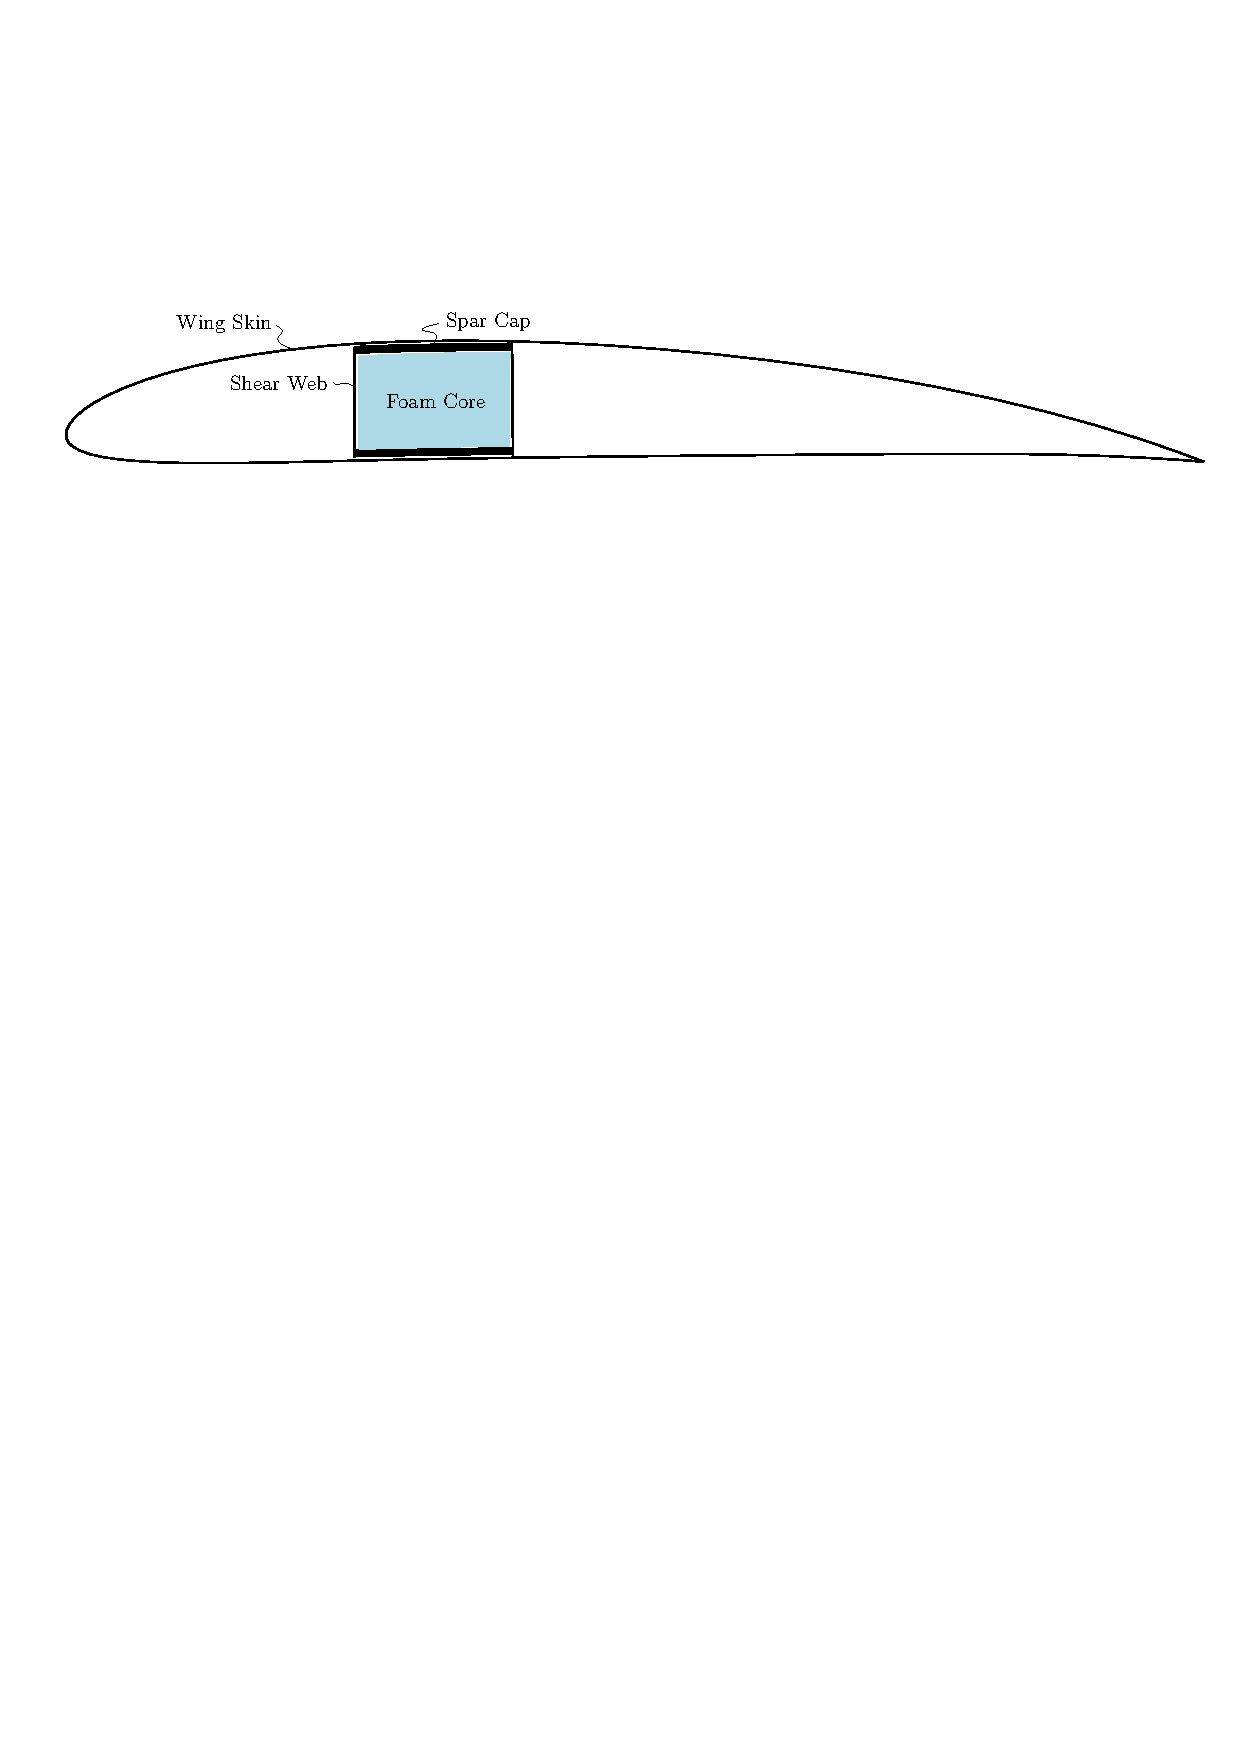
\includegraphics[width=0.9\textwidth]{capspar.pdf}
    \caption{\textbf{Cross sectional view of a cap spar.}}
	\label{f:capspar}
	\end{center}
\end{figure}

The spar dimensions are sized such that the material stresses are not exceeded under a 3.5 g-load,

\begin{equation}
    \sigma_{\mathrm{CFRP}} \geq \frac{\mathcal{M}_{\mathrm{root}}}{S_{y_{\mathrm{spar}}}}
\end{equation}

The root wing moment $\mathcal{M}_{\mathrm{root}}$, is calculated assuming a distributed load along the wing span that scales with the local chord.\cite{bending}
A constant tapered wing is assumed.  
This wing sizing model leverages the GP wing sizing model used by Burton and Hoburg.\cite{burton_solar_2017} 

A simple drag model is used for the aircraft, 

\begin{equation}
    C_D \geq CDA + c_{d_p} + \frac{C_L^2}{\pi e AR}.
\end{equation}

where the profile drag coefficient $c_{d_p}(C_L, Re)$, is calculated from a representative wing polar. 
The combined drag and wing loading models allow the aspect ratio to be optimized, trading structural integrity with aerodynamic performance. 

\subsection{Takeoff and Landing Models}

The takeoff model was adapted from Raymer's takeoff equations to fit a GP compatible form.  Using equations of motion the takeoff state can be expressed

\begin{equation}
    T - D - \mu(W_{\mathrm{MTO}} - L) = \frac{W_{\mathrm{MTO}}}{g} \frac{dV}{dt}.
\end{equation}

This can be simplified to 
\begin{align}
    \frac{dV}{dt} &= g \left( \frac{T}{W_{\mathrm{MTO}}} - \mu \right) - \frac{g}{W_{\mathrm{MTO}}} \left( \frac{1}{2} \rho S V^2 (C_{D_g} - \mu C_{L_g})\right) \\
    \label{e:todiff}
    \frac{dV}{dt} &= \frac{1}{A-BV^2}
\end{align}

The takeoff ground run distance can then be expressed by taking the integral of Equation~\ref{e:todiff} to achieve

\begin{equation}
    \label{e:to}
    S = \frac{1}{2B} \ln{\frac{A}{A-BV^2}} 
\end{equation}

The natural log function can be approximated to make Equation~\ref{e:to} GP-comptible by 

\begin{equation}
    \ln{\frac{A}{A-BV^2}} \approx \num{5.6e-4} A^{-6.04} (BV^2)^{6.04} + 1.0 A^{-0.001} (BV^2)^{0.001} + \num{7.5e-4} A^{-1.276} (BV^2)^{1.275}
\end{equation}

with an average log error of 0.06\%.  The terms $A$, and $B$, are constrained by

\begin{align}
    \frac{T}{W_{\mathrm{MTO}}} &\geq \frac{A}{g} + \mu \\
    B &\geq \frac{g}{W_{\mathrm{MTO}}} \frac{1}{2} \rho S C_{D_g}
\end{align}

where the $\mu C_{L_g}$ term is neglected as a conservative approximation for $B$ to preserve GP-compatibility. 

\section{Market Analysis}

\section{Conclusion}

\bibliography{biblibrary}
\bibliographystyle{aiaa}

\end{document}

